\chapter{ADDITIONAL RADIOGRAPHIC EVIDENCE AND METRICS}
\label{app:appendix_a}

\section{ARCADE Dataset Distribution Details}
The Automated Regional Coronary Angiography and Diagnostic Evaluation (ARCADE) benchmark provides standardized subsets used for training and evaluating the three platform models:
\begin{itemize}
    \item \textbf{Syntax Vascular Tree Track:} 1,000 training images and 200 validation images with complete vessel segmentation annotations across major epicardial coronary trunks and branches.
    \item \textbf{Stenosis Track:} Annotated regions of interest delineating lumen boundaries, eccentric plaques, and focal narrowing percentages.
\end{itemize}

\section{Additional Viewplates of 3D Coronary Artery Interior}
Figure~\ref{fig:appendix_cross_sections} illustrates the individual calibrated cross-sections generated at proximal reference, minimal lumen area, and distal reference locations along the Left Anterior Descending artery for case \texttt{CAI-E6C66811}.

\begin{figure}[H]
\centering
\begin{subfigure}[b]{0.32\textwidth}
    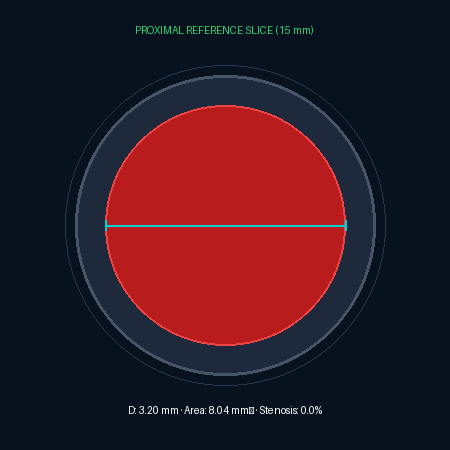
\includegraphics[width=\textwidth]{figures/03_proximal_cross_section.png}
    \caption{Proximal Reference ($3.00\text{ mm}$)}
\end{subfigure}
\hfill
\begin{subfigure}[b]{0.32\textwidth}
    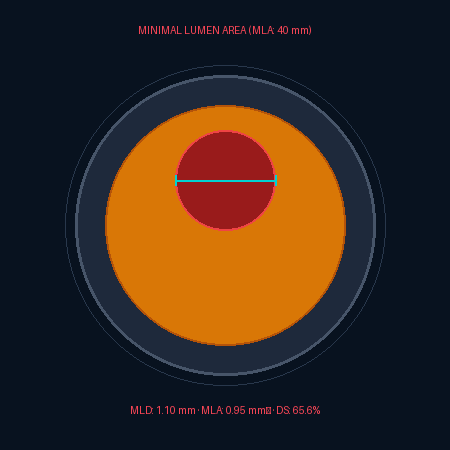
\includegraphics[width=\textwidth]{figures/04_minimum_lumen_cross_section.png}
    \caption{MLA Section ($1.48\text{ mm}$)}
\end{subfigure}
\hfill
\begin{subfigure}[b]{0.32\textwidth}
    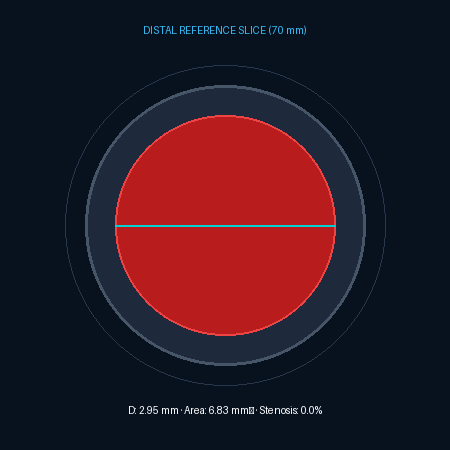
\includegraphics[width=\textwidth]{figures/05_distal_cross_section.png}
    \caption{Distal Reference ($3.64\text{ mm}$)}
\end{subfigure}
\caption{Cross-Sectional Circular Lumen and Wall Slices Generated by the QCA Geometry Engine}
\label{fig:appendix_cross_sections}
\end{figure}
